\documentclass[%
% if you want to use pdflatex, uncomment the following line
%pdftex
% if you have difficulties with fonts uncomment the following line
%notimes
]{algotel}
\usepackage[latin1]{inputenc}
\usepackage{ mathrsfs }
\usepackage{mathtools}  
\usepackage{amsmath}
\usepackage{relsize}
\usepackage{lmodern}
\usepackage{slantsc}
\usepackage{amssymb}
\usepackage{tabulary}
\usepackage{booktabs}
\usepackage{multicol}
\usepackage{blindtext}
\usepackage[francais]{babel}

\newcommand{\exedout}{%
  \rule{0.8\textwidth}{0.5\textwidth}%
}

\author{Nicolas Herbaut\addressmark{1}\addressmark{2}\thanks{The work performed for this paper has been partially funded by the FP7 IP T-NOVA European Project (Grant Agreement 619520) and the FUI French National Project DVD2C}{\ }
  \and Daniel N�gru\addressmark{1}}


\title[]{D�ploiement d'un chaine de service de livraison de contenu multimedia sur une infrastructure d'op�rateur bas�e sur SDN-NFV}

\address{\addressmark{1}Univ. Bordeaux, LaBRI, UMR 5800, F-33400 Talence, France
\addressmark{2}Viotech Communications, Versaille, France

}


\keywords{SDN, NFV, Service Chaining, Content Delivery, CDN ISP Collaboration}

\begin{document}
\maketitle

\begin{abstract}
La consommation de videos "over the top" a chang� la donne pour les acteurs du monde de la livraison de contenu. La chaine de valeur a gliss� progressivement en faveur des fournisseurs de contenus et des r�seaux de livraison de contenu et au d�triment des fournisseurs d'acc�s.
Notre contribution propose un nouveau mod�le de collaboration entre ces diff�rents acteurs par la cr�ation d'une plateforme o� sont d�ploy�es des cha�nes de service de distribution de contenu. Nous �tudions en particuliers les solutions de placement de ces fonctions r�seaux sur un substrat de serveur virtualis�s au sein d'un r�seau respectant l'approche Software Defined Network (SDN) dans lequel sont d�ploy�es des infrastructures de virtualisation de fonction r�seau (NFV).
\end{abstract}

\section{Introduction}
Real-time entertainment (video and audio streaming) is the number one service on the current Internet: it accounts for 68.90\% of the Downstream Peak Period Traffic in North America in Q2 2015  \cite{sandvine_2015}. As the Internet was not originally designed for streaming high quality video, delivering this massive amount of content is a challenging task. 

One solution to mitigate those issues is to use Content Delivery Networks (CDN). 
CDNs have been created to improve network performance for end-users while at the same time limiting the need for Content Providers (CP) to own an infrastructure \cite{pathan2014cloud}.
By deploying servers in strategic locations, CDN Providers assign users to a close-by server, thus reducing hop count and avoiding congestion occurrences.

In this very competitive market, the majority of ISPs are being kicked out of the video delivery value chain and is struggling to minimize the drop in their revenues \cite{wulf_carrier_2010}.  
However, even if their business role in the delivery part is challenged by CDNs, ISPs still hold a valuable asset: they can manage the whole network, i.e., the complete routing process end-to-end. 

The envisioned solution is a collaboration model for ISP and CDN around a Network Function Virtualization (NFV) architecture.
We propose a solution where ISPs can manage a NFV infrastructure where CDNs can run their caching software as NFVs through a virtual CDN (vCDN) network function.
It is a win-win approach since CDNs can expand their coverage dynamically without buying new servers and ISPs can increase their revenue by billing them while reducing inter-AS traffic.

The rest of the paper is organized as follows.
Section~\ref{sec:architecture} describes the architecture of the solution, while Section~\ref{sec:model} details the model used to optimize the placement of the whole content delivery service. Section~\ref{sec:result} presents the results of the modelization. We conclude the paper in Section~\ref{sec:conclusion}.

\section{A NFV/SDN platform for virtual CDN deployment in the ISP's network\label{sec:architecture}}

In order to overcome the CDN-ISP collaboration challenges, we propose a Virtualized Infrastructure solution capable of matching ISP's connectivity "supply" with the CDN's connectivity "demand", towards a win-win approach.

Our proposal, as depicted in Figure~\ref{fig:overlay}, aims at instantiating a Network Function Virtualization (NFV) platform within the ISP Network capable of hosting, among others, Virtual CDN (vCDN) services. 

This platform is distributed amongst several NFV infrastructure points of presence (NFVI-POP), at the edge of the network. 
NFVI-POPs contains racks of servers that provide resources (CPU, RAM, HDD) to run virtual Network functions on.

For the network part, we consider using SDN at the ISP level, allowing a virtually centralized management of the control plane.
By allowing packets to flow along reserved virtual routes throughout the ISP network, the solution allows predictability of both bandwidth and latency between the End-User and the vCDN caching server. 

By allowing compute and network resources beeing allocated to third party on its network, ISPs are capable of contracting Service Level Agreement (SLA) with the CDN to run vCDN.

While an SLA is a good way for CDNs to formulate their business needs, it doesn't specify technically how service is implemented. 
The canonical representation of Content Delivery Service is depicted Figure~\ref{fig:canonical}, where two distinct flows emerge from the source $s$. On one hand, we have the $s\rightarrow CDN$ flow which represents the traditional path to content delivery: packets flow through the ISP network and reach the seperate CDN network. On the other hand, the $s \rightarrow vCDN$ flow is targetted at an ISP operated POP located within its network.
The latter flow has tighter network constraints (low delay, high bandwidth) and can hence deliver better quality videos.

While traditionnal DNS redirection methods can be used to decide where to steer trafic, Operators can benefit from an SDN approach to control traffic with more granularity.
One of the drawback of SDN hovever, is that its southbound interfaces \cite{openflow} only accept L1-L4 rules, limiting greatly the possibilities left by the CDN to choose the righ server.
To mitigate this issue, we propose using a Virtual Home Gateways (vHG) \cite{vhgpaper}. 
vHG are virtual appliances that outsource traditional physial Home Gateway's Network Functions to the cloud, leaving a simple L2 bridge on the user premicises \cite{vhg paper}. 
In our usecase, vHG can be seen as a transit function able to flag outgoing flows according to L5-L7 rules, like HTTP URL for instance.
vHG can seggregate traffic targetted to vCDN from the one targetted to CDN allowing packets to follow distinct routes with distinct network caracteristics.

The resulting service can now be seen as a Service Chain depicted in Figure~\ref{fig:vhg}.
The ISPs need to embed the service chain generated from the CDN SLA into their substrate network. 
This problem is known as Service Chain Embedding \cite{service chain} where we need to map a service graph $G^{S}=(N^{S},E^{S})$ to a substrate graph $G=(N,E)$ representing the real ISP network. Figure~\ref{fig:service-mapping} shows such a mapping.

SLAs varies in the amont of physical resources needed and can be very demanding sometimes. In this context, it can be quite challenging for the ISPs to map a vNF or a Route to their



\begin{figure}
\centering
\begin{minipage}{0.45\textwidth}
\centering
	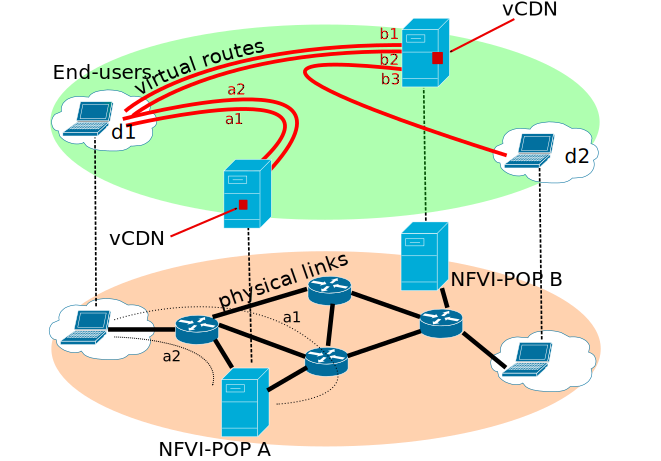
\includegraphics[width=1\textwidth]{fig/overlay.pdf}
	\caption{ISP's Virtualized Network
    \label{fig:overlay}}
\end{minipage}\hfill
\begin{minipage}{0.45\textwidth}
\centering
	\includegraphics[width=1\textwidth]{fig/sla-service-vne.png}
	\caption{ From SLA to Service Embedding
    \label{fig:sla-service-vne}}
\end{minipage}
\end{figure}


\begin{figure}
\centering
\begin{minipage}{0.20\textwidth}
\centering
	\includegraphics[width=1\textwidth]{fig/service.pdf}
	\caption{Service Canonical Representation
    \label{fig:canonical}}
\end{minipage}\hfill
\begin{minipage}{0.335\textwidth}
\centering
	\includegraphics[width=1\textwidth]{fig/service_vhg.pdf}
	\caption{Service implementation using Virtual Home Gateway
    \label{fig:vhg}}
\end{minipage}
\begin{minipage}{0.33\textwidth}
\centering
	\includegraphics[width=1\textwidth]{fig/lb-service.pdf}
	\caption{Transformed service with Load Balanced Home Gateways
    \label{fig:vhg-lb}}
\end{minipage}
\end{figure}

\begin{figure}
	\center
	\includegraphics[width=0.95\textwidth]{fig/service-mapping.pdf}
	\caption{Mapping of a Service Chain
    \label{fig:service-mapping}
    }
\end{figure}


\section{Model}

minimize 

\begin{equation} \label{eq1}
\begin{split}
\max_{
\!\mathsmaller{x \in \mathscr{T} }}{\mathscr{D}(s,x)} 
											 &=\max_{\!\mathsmaller{x \in \mathscr{T}} }{
			\sum_{
			\!\mathsmaller{
			(i,j)\in\mathscr{P}^{S}(s,x)
			}
			}{\mathscr{D}_{\mathscr{M}}(i,j)}}\\
											&=\max_{x \in \mathscr{T} }{
			\sum_{
			\!\mathsmaller{
			(i,j)\in\mathscr{P}^{S}(s,x)
			}
			}}{\quad\sum_{
			\!\mathsmaller{
			{(a,b)\in\mathscr{P}^{S}_{\mathscr{M}}(i,j)}
			}
			}{d_{a,b}\times y_{a,b}^{i,j}}}\\
\end{split}	
\end{equation}

\begin{equation}
		\sum_{u\in N} x_u^{i}=1, \forall i \in N^{S}
\end{equation}


\begin{equation}
	\sum_{i \in N^{S} } x_{j}^{i} \times c_{i}^{S} \leq c_{u}, \forall u \in N		
\end{equation}

\begin{equation}
	\sum_{(i,j)\in E^{S}}{y_{u,v}^{i,j}\times b_{i,j}^{S}} \leq b_{u,v}, \forall (u,v) \in E
\end{equation}

\begin{equation}
	y_{u,v}^{i,j}\times d_{u,v} \leq d_{i,j}^{S}, \forall (u,v) \in E, \forall (i,j) \in E^{S}
\end{equation}


\begin{equation}
\sum_{v \in N}{y_{u,v}^{i,j}-y_{v,u}^{i,j}} = x_{u}^{i}-x_{u}^{j}, \forall (i,j) \in E^{S}, \forall u \in N
\end{equation}


\begin{equation}
y_{u,v}^{i,j}+y_{v,u}^{i,j} \leq 1, \forall (u,v) \in E, \forall (i,j) \in E^{S}
		s
\end{equation}

  
\begin{table}[htbp]\caption{Notations}
\begin{center}% used the environment to augment the vertical space
% between the caption and the table
\begin{tabular}{r c p{4cm} | r c p{4cm} }
\toprule{}

$\mathscr{M}$ & $\triangleq$ & maps a service graph $G^{S}=(N^{S},E^{S})$ to a substrate graph $G=(N,E)$.
& $\mathscr{P}^{S}(i,j)$ & $\triangleq$ & the set of edges $e\in E^{S}$ that links $i \in N^{S}$ to $j \in N^{S}$\\

$\mathscr{P}^{S}_{\mathscr{M}}(i,j)$ & $\triangleq$ & the set of edges $e\in E$ that links $u$ to $v$ with $i \xrightarrow{\mathscr{M}} u$ and $j \xrightarrow{\mathscr{M}} v$&
$\mathscr{D}_{\mathscr{M}}(i,j)$ & $\triangleq$ & the total substrate delay for mapping $\mathscr{M}$ for $(i,j) \in E^{S}$ \\

$\mathscr{T}$ & $\triangleq$ & the set of terminal nodes of the service chain.&
$i \xrightarrow{\mathscr{M}} u$ & $\triangleq$ & network function $i\in N^{S}$ is mapped to the $u\in N$ for mapping $\mathscr{M}$ \\

$y_{u,v}^{i,j}$ & $=$ & \(
	\left \{
		\begin{array}{p{0.5cm}p{2.5cm}}
			1,  & if link $(i,j) \in E^{S}$ \\ & is mapped on substrate link $(a,b)\in E$ \\
			0,  & \text{otherwise} 
		\end{array}
	\right.\)&



$x^{i}_{u} $ & $=$ & \(
	\left \{
		\begin{array}{p{0.5cm}p{3.5cm}}
			1,  & \text{if $i \xrightarrow{\mathscr{M}} u$} \\
			0,  & \text{otherwise} 
		\end{array}
	\right.\)\\
	
$d_{a,b}$ & $\triangleq$ & the delay for edge $(a,b)\in E$ &
$d^{S}_{i,j}$& $\triangleq$ & the maximum delay on $(i,j) \in E^{S}$ admissible for chain $G^{S}$.\\

$b^{S}_{i,j}$& $\triangleq$ & the required bandwidth on $(i,j) \in E^{S}$ for chain $G^{S}$'s operation.&
$b_{u,v}$& $\triangleq$ & the available bandwidth on edge $(u,v) \in E$  of the substrate\\

& & & $s$ & $\triangleq$ & the starting node of the service chain.\\




\bottomrule
\end{tabular}
\end{center}
\label{tab:TableOfNotationForMyResearch}
\end{table}


\nocite{}
\bibliographystyle{alpha}
\bibliography{algobib}



\end{document}
